%% Overleaf			
%% Software Manual and Technical Document Template	
%% 									
%% This provides an example of a software manual created in Overleaf.

\documentclass{ol-softwaremanual}

% Packages used in this example
\usepackage{graphicx}  % for including images
\usepackage{microtype} % for typographical enhancements
\usepackage{minted}    % for code listings
\usepackage{amsmath}   % for equations and mathematics
\usepackage{placeins}
\usepackage{pdflscape}
\setminted{style=friendly,fontsize=\small}
\renewcommand{\listoflistingscaption}{List of Code Listings}
\usepackage{hyperref}  % for hyperlinks
\usepackage[a4paper,top=4.2cm,bottom=4.2cm,left=3.5cm,right=3.5cm]{geometry} % for setting page size and margins

\graphicspath{{images}}

% Custom macros used in this example document
\newcommand{\doclink}[2]{\href{#1}{#2}\footnote{\url{#1}}}
\newcommand{\cs}[1]{\texttt{\textbackslash #1}}

% Frontmatter data; appears on title page
\title{Imagine analysis pipeline\\User manual}
\version{1.0.0}
\author{IMAGINE Project}
\softwarelogo{
\includegraphics[width=8cm]{logo}}

\begin{document}

\maketitle

\tableofcontents
\newpage

\section{Introduction}
The Imagine analysis pipeline automatically extracts features from biofilm images, identifies patterns in three-dimensional data and classifies images based on a selected target. Here we present the use when the target is the name of the strain and the classification process is used to determine which bacterial strain each image represents.

\section{Image requirements}
As input we use 3D images (z-stacks) of biofilms consisting of several image layers. They must be saved in tif format, other formats are currently not compatible with the pipeline.

In case of Zeiss LSM10 microscope high-throughput imaging, the images at different positions of the sample can be acquired in such a way that the images are saved in one file. The images for further analysis must be separated into separated tiffs (one image represents only one position, which includes all images of a 3D stack). This can be done using open source software \doclink{https://imagej.net/software/fiji/}{ImageJ FIJI} with a provided ImageJ script for splitting and converting images from lsm files (Zeiss microscopes) (Figure~\ref{fig:script}).

The execution of the Imagine pipeline depends heavily on the information contained in the image names, which should follow the example below.

Scheme for image naming:\\
<DT>\_s\_<SP>\_st\_<ST>\_p\_<WC>\_pos<WP>\_tm\_<GT>\_ch\_<CH>\_z\_<LD>

\begin{itemize}
	\item \textbf{DT} - date
	\item \textbf{SP} - species
	\item \textbf{ST} - strain
	\item \textbf{WC} - well coordinates
	\item \textbf{WP} - well position
	\item \textbf{GT} - growth time
	\item \textbf{CH} - channel
	\item \textbf{LD} - layer distance
\end{itemize}

Example image name:\\ 07112023\_s\_Lm\_st\_L1823\_p\_F02\_pos005\_tm\_24\_ch\_Syto9\_z\_21

Explanation of the name:
\begin{itemize}
\item 07112023: date in DDMMYYYY format
\item s\_Lm: s\_ indicates the species, Lm means Listeria monocytogenes 
\item st\_L1823: st\_ denotes the strain, L1823 is the name of the strain 
\item p\_F02: p\_ denotes the well coordinates on the 96-well plate, F02 is the actual position on the 96-well plate 
\item pos005: pos denotes the measured position within the individual well, e.g. position 5 in well F02 
\item tm\_24: tm\_ stands for the measurement time, 24 means that the images were taken after 24 hours of biofilm growth 
\item ch\_Syto9: ch\_ denotes the channel, Syto9 is the name of the dye and filter used 
\item z\_21: z\_ denotes the number of layers in the 3D image, which also reflects the distance between two consecutive layers.
\end{itemize}


The image names are parsed on the back-end. Thus, following the naming structure is very important. Any deviation from the described pattern will result in processing failure.

The renaming process can be carried out semi-automatically by the \doclink{https://www.advancedrenamer.com/}{software}, or by user-defined scripts. Examples and the user manual are available \doclink{https://www.advancedrenamer.com/user\_guide/v3/complete\_guide}{here} together with graphical representations. 


\begin{figure}
	\centering
	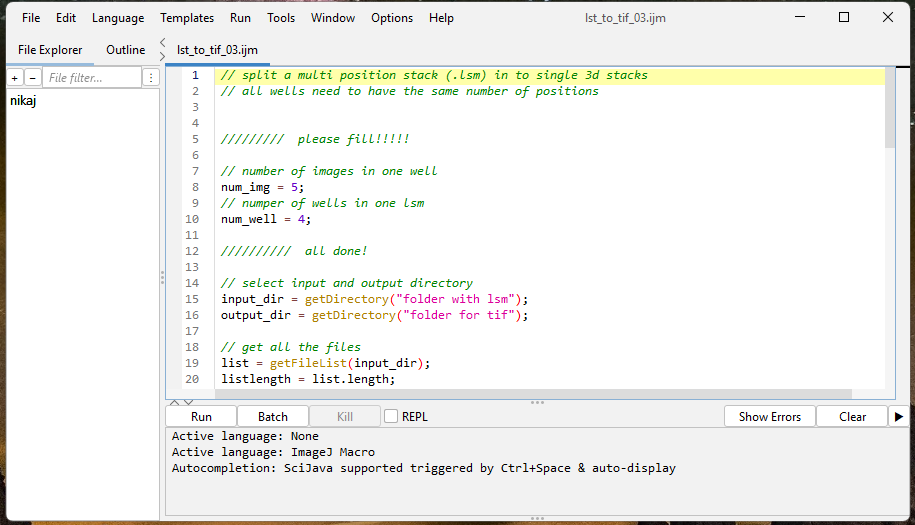
\includegraphics[width=\textwidth]{script}
	\caption{\label{fig:script} The script enables the conversion of an lsm file with several 3D stacks taken in different wells into single 3D stack per position (one-position­-one-set of images – one 3D stack) in tif format. The script is loaded by dragging it onto the ImageJ; once it opens, the number of images per well and the number of wells in which images are captured must be adjusted. This script also relies on the image naming shown below. If you do not follow these, the script will not work.}
\end{figure}

\FloatBarrier

\section{PC Requirements}

The Imagine pipeline is designed to run on both Windows and Unix-based systems, or more generally on any system that supports Docker. Hardware requirements include at least two computing cores (CPUs) and 4 gigabytes of ram. The files required to run the pipeline are approximately 500 MB in size, and 1 GB of memory may be required to run the analysis smoothly.

Level required:
\begin{itemize}
	\item User level of windows environment navigation. Acquaintance with command line in Windows, basics available \doclink{https://www.geeksforgeeks.org/most-useful-cmd-commands-in-windows/}{here}.
	\item Acquaintance with Docker environment, basics available \doclink{https://www.docker.com/blog/getting-started-with-docker-desktop/}{here}.
\end{itemize}

\subsection{Docker installation}
A Docker host daemon is required to build Docker images. The easiest way to meet this requirement is to install the Docker Desktop application.

\begin{enumerate}
	\item Download and install the Docker Desktop application from the website. This might take a minute, depending on your system and will require you to restart your computer. \doclink{https://docs.docker.com/desktop/install/windows-install/}{Link Windows} | \doclink{https://docs.docker.com/desktop/setup/install/linux/}{Link Ubuntu Linux}.
	\item Start Docker Desktop by double-clicking on the Docker icon in the Start menu. It might run in the background and you might need to bring it to the front from the tray (bottom right corner).
\end{enumerate}

\begin{figure}
	\centering
	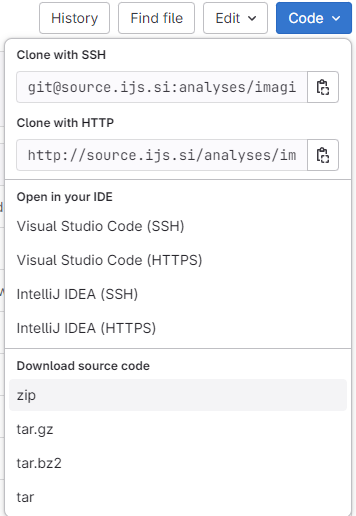
\includegraphics[width=0.5\textwidth]{git}
	\caption{\label{fig:git} Downloading the source code. (i) Click "code" (ii) Click on “zip” option in the "download source code" section of the dropdown. (iii) Save the zip file to Desktop.}
\end{figure}

\subsection{Building the Docker image}

The next step is to build the Imagine Docker image.
\begin{enumerate}
	\item Download "imagine-main.zip" from the imagine git website (see Figure~\ref{fig:git}).
	\item Extract "imagine-main.zip" into the imagine-main (you can rename it if you want) folder on your desktop. 
	\item Navigate into the folder that you extracted the zip file into, right-click and select "open in terminal" to start the terminal in the "imagine-main" folder. Link to “open in terminal” can be hidden also in “show more options”.  If these options are not available on your system we suggest extracting the downloaded file onto C:/, open cmd and navigate to the folder using command cd e.g. cd C:/path/to/my/folder. Cmd can be found by typing “cmd” in Windows search and is run by clicking on “Command Prompt”. 
	\item Connect to the internet prior to running the build command. 
\end{enumerate}

Once the above steps are done, write or copy the following command into the terminal to build a Docker image specifically created for running the Imagine project analyses.

For Windows users:
\begin{minted}{bat}
c:\my-download-folder\imagine> build-and-verify.bat
\end{minted}

For Linux users:
\begin{minted}{sh}
# to make the file executable
(/my-download-folder/imagine) $ chmox +x build-and-verify.sh 
(/my-download-folder/imagine) $ ./build-and-verify.sh
\end{minted}

Once the Docker image is built and verified (it takes a while), you can run analyses as described below. 
The Docker image will not need to be rebuilt unless changes are made to the Imagine pipeline scripts.

You can close the Docker desktop application but leave it running in the background (you will see an icon in the taskbar indicating that the Docker daemon is still running and ready to run containers). You can close the terminal window if you do not intend to continue or leave it open to run the Imagine pipeline.


\section{Preparation of data for running the Imagine pipeline}

Before executing the command to calculate features you need to: 
\begin{enumerate}
	\item Prepare a folder with your input images, e.g. create a folder example\_images on the desktop, and remember the path or address of the folder, e.g. /c/Users/my\_name/Desktop/example\_images).
	\item Create a folder in which you want to save the calculation results. For example, create the subfolder results\_example on the desktop and make a note of the path or address, e.g.\\ /c/Users/my\_name/Desktop/imagine/results\_example.
	\item (optional) Change the voxel dimensions if necessary: To do this, go to imagine-main/src, find the feature generator script and change the following part as desired: \\
	\# constants voxel\_size = 0.13 * 0.13 * 0.5 pixel\_area = 0.13 ** 2. If you make changes to the feature generator code, you must recreate the Docker image as described above.
	\item Open the folder "imagine-main" (or the name you chose when unzipping the zip file). Search for the file with the name “.env”.
\end{enumerate}

You will need to replace the path to the images in the .env file: \\
"/c/Users/my\_name/Desktop/example\_images" with the path or address where your images are located. You can check this in the address bar of the window when the folder with the images is open. This address needs to be changed slightly to be compatible with Docker by following the rules below: change "\" to "/" and remove ":" as in the following example: 

c:\\my\_folder\\test\_images, you need to write it as /c/my\_folder/test\_images. Make sure that you do not change the text after the ":".

One must replace "/c/Users/my\_name/Desktop/imagine/results\_example" with the corresponding path if you have created the subfolder in a different location than described above. The address must be changed as described above. Again, make sure that you do not change the text after the ":".

Open the file and change the paths in the .env file:

\# change these paths so that they point to your data and desired results folder\\
IMAGINE\_IMAGES=/c/Users/my\_name/Desktop/example\_images\\
IMAGINE\_RESULTS=/c/Users/my\_name/Desktop/imagine/results\_example

Alternatively, you can also create your own file with the information about the paths. Save this file in the “imagine-main” folder. If you run generate\_features or learning\_benchmark, you must specify the name in the command (see below). While in the "imagine-main" folder (or whatever name you picked when you extracted the zip file) open the terminal in this folder as described above (right click, then "open in terminal"). Additionally, the Docker daemon must be running (there should be an icon in the taskbar). If it is not, open the Docker Desktop application as described above.


\section{Generating features using the Imagine pipeline}

To generate features with the Imagine pipeline, run the following command in the terminal (the parts in<> must be replaced as described above and below and <> as well (see examples below):

\begin{minted}{sh}
docker compose run --rm datafile.tsv generate_features
\end{minted}

If you are not using an .env file but your own file, change the command accordingly:

\begin{minted}{sh}
docker compose 
  --env-file myownfilename.txt 
  run 
  --rm imagine 
  datafile.tsv generate_features
\end{minted}

For the examples above, the command is:
\begin{minted}{sh}
docker compose run 
	--rm imagine 1 
	datafile.tsv 10 generate_features
\end{minted}


And, if you use your own file with paths:
\begin{minted}{sh}
docker compose 
  --env-file test_paths.txt run 
  --rm imagine 1 datafile.tsv 10 generate_features
\end{minted}

The parameter “1” determines the parallelization rate — a higher parallelization (should not exceed the number of CPU cores in your computer) works faster, but consumes more resources of the computer, while a lower parallelization (1) works slower, but should also be completed on machines with fewer resources.

The parameter “10” determines how many of the top features are used in the visualizations.

If you want to test the software, you can use test images (which are supplied with the software) by executing the test\_images folder as:
\begin{minted}{sh}
docker compose run --rm imagine-test-generate-features
docker compose run --rm imagine-test-learning-benchmark
docker compose run --rm imagine-test-data-visualization
\end{minted}


The main output of this step is \textbf{datafile.tsv}, where all calculated features are available for review.
Once the process is complete, check the results folder and in particular the datafile. 
In the first column of the data file, all analyzed images should be listed by name. If some images are missing, check the format of the missing images. 

An example of what kind of results you can expect can be found in the imagine-main/results\_example folder that belongs to the pipeline.

The file datafile.tsv can be opened with Excel for checking. If the file becomes too large for Excel, selected rows of the table can be exported to csv and opened with Excel to check the calculations more intuitively:
Open the command prompt as described above. 
Navigate to the folder with the results using the cd command as described above. Then use the command:
\begin{minted}{sh}
type datafile.tsv | 
Select -First 15 > first_15_rows_of_datafile.csv
\end{minted}


The features from the data file are now prepared for running the classification model.

How features are calculated is described in the last chapter of the manual and in the attached table. Further details can be found in the code itself. Many examples are also given in the manuscript based on the use case of Listeria biofilms.




\section{Classification using the Imagine pipeline}

The command for comparison of the classifiers (benchmark) is as follows (the <> sections must be replaced as above):

\begin{minted}{sh}
docker compose run 
	--rm imagine 
	datafile.tsv learning_benchmark	
\end{minted}

For example:
\begin{minted}{sh}
docker compose run 
	--rm imagine 1 
	datafile.tsv 10 learning_benchmark 
\end{minted}

The parameter “1” determines the parallelization rate — a higher parallelization (should not exceed the number of CPU cores in your computer) works faster, but consumes more resources of the computer, while a lower parallelization (1) works slower, but should also be completed on machines with fewer resources.

The parameter “10” determines how many of the top features are used in the visualizations.

For the classification comparison, the set of given images is randomly divided by the software into a training set and a prediction set. The training set is used to train the model and the prediction set is used to test how accurately the names of the strains can be predicted based on the trained model. These results show us how successfully the strains could be predicted.

The results of the comparison of the classifiers are contained in three different files:
\begin{itemize}
	\item classification\_all
	\item classification\_no\_counts\_features
	\item ablation\_ranking\_all
	\item rankings\_date
	\item rankings\_label	
\end{itemize}

Label here corresponds to the string that follows \_st\_ in the name of the image, in this case strain name. The classification target is the property predicted by the classifier, and in this case the target corresponds to the label, i.e. the name of the strain. The date refers to the exact date on which the experiment took place and is linked to the biological replicas. The date is also indicated in the name of the image (see naming convention). 

Under some circumstances (most notably low available memory) some of the models (AutoGluon) can unfortunately crash the container, however, the software is designed in such a way to store intermediary results so most of the computation will not be wasted. If the software exits prematurely, you can try to rerun it and it should pick up where it left off. In case it stops again, try closing other applications that might be using up the available memory. In the case where a model will not complete even after several tries you can disable it using the instructions provided below.

Disabling individual models:
The file that determines which models will be used in the benchmark is src/feature\_ranking\_lite.py. If you wish to disable some of the models locate the line 268; starting from there the following lines should include a defintion of which models are used, e.g., as such:

\begin{minted}{python}
models = {
	'dummy': DummyClassifier(),
	'decisiontree': tree.DecisionTreeClassifier(),
	'logistic': LogisticRegression(),
	'rf': RandomForestClassifier(),
	'xgb': XGBClassifier(
	        n_estimators=100,
			max_depth=3, 
			learning_rate=1, 
			objective='binary:logistic'),
	'gridsearch': GridSearchCV(
			KNeighborsClassifier(), 
			parameters, 
			n_jobs=PARALLELISM),
	'autogluon': TabularPredictor(label="label"),
}
\end{minted}

Any model can be disabled by placing a hash symbol \# immediately before its defintion. For example, to disable "autogluon":
\begin{minted}{python}
#'autogluon': TabularPredictor(label="label"),
\end{minted}

After any such modification in the selected models, the image should be rebuilt by using:
\begin{minted}{sh}
docker compose build imagine
\end{minted}


\subsection{Explanations of individual files}

\subsubsection{Classification\_all and classification\_no\_counts\_features}

These two files summarize the results of classification by selected machine learning algorithms. The columns from left to right are:
\begin{itemize}
	\item tag – has value RESULT and it has been used for parsing, but is currently not active
	\item upsampling – has value 1 
	\item model - type of classifier, random forest, etc. and dummy classifier as sanity test 
	\item n\_components - number of input features 
\end{itemize}


The classifiers can be fed with all features, currently there are 2700, or the number of features can be reduced beforehand by the SVD decomposition model, which selects the features it considers important and outputs the number of features the user selects - here we reduce the number of features by a factor of two; when comparing the accuracy for the reduced data, you should bear in mind that the features selected by SVD are not the same for all dimensions, which means that the model can be fed with different features and therefore produce different results.
\begin{itemize}
	\item fold – number of iterations (repetitions)
	\item accuracy - number of correct predictions (key result of the comparison)
	\item test\_set - name of the strains (labels) used for the classification test, 
	\item thr\_features – TRUE if features with threshold are included and FALSE if features with threshold are excluded; for each number of n\_components results for TRUE and FALSE are given; for n\_components 580 we have only FALSE (all features except the one with threshold) and for 2700 only TRUE (because all features include the one with threshold) – so 580 and 2700 should thus be considered and compared together
\end{itemize}

For the task of classifying biofilm images by strain name, we choose the classifier random forest. The following files contain information derived exclusively from classifications based on random forest.

\subsubsection{Ablation\_ranking}
The report shows how model accuracy changes as features are added incrementally. Determining the highest accuracy for a dataset shows how many features are required to classify the strains. For interpretation, we recommend selecting the number of features that gives the highest accuracy and then using the same number of features with the highest score to explain which ones contribute the most to the classification.
For example, in ablation\_ranking we find that the number of features with the highest accuracy is 81; then we go to the ranking file and select 81 features with the highest score for further interpretation.

\subsubsection{Rankings\_label and rankings\_date}
Label here corresponds to the string that follows \_st\_ in the name of the image, in this case strain name, and in the classification we call the property that is predicted, the target here is either the label (strain) or the date.

For each feature calculated, the strength of its relationship to the target is indicated, with larger values indicating that the feature was more important in predicting strain and vice versa (rankings\_label). We also provide rankings for date prediction (rankings\_date) to account for features that may vary as a consequence of repeating the experiment on different days (likely due to the methodology or variability of the biological system under study). This is crucial when we provide multiple images from different days (biological replicates) for a single strain to the model, as the variation within a single day is often less than between different days. If the model relies on features describing biofilm characteristics that are tied to specific dates rather than strains across different dates, it may lead to bias and poorer results. We suggest that the features included in rankings\_label and rankings\_date are compared and that the high-ranking, overlapping features are not considered when explaining the complexity of the system.


\section{Visualisations of the comparisons of the performance of classifiers and the ablation ranking}
The results of the performance comparison between the selected classifiers (based on calculations from the classification\_all and\\ classification\_no\_counts\_features) and the ablation ranking (ablation\_ranking) are now visualised to facilitate the interpretation of the results. These are found in the folder “Visualizations”.

\section{Examples of applications of the developed pipeline to optimise the experimental setup or to use the pipeline to predict other properties related to biofilm characteristics}

\subsection{How do you use the pipeline if you want to link biofilm features to properties other than the strain name?}

The easiest way is to replace the string after \_st\_ in the image name with the desired property. For example, to associate biofilm features with clinical relevance, replace the string after \_st\_ (strain name) with CI (clinically relevant) or CNI (clinically not relevant) based on the epidemiology of the strain. Then run the pipeline as usual.

\subsection{Using the pipeline to determine whether the number of layers in a 3D image affects classification performance}
The number of layers in the 3D images can be reduced with the command from the pipeline:
\begin{minted}{sh}
docker compose run 
	--rm imagine datafile.tsv 
	reduce_layers <initial number of layers>
\end{minted}

To reduce the layers from 21 to 11, you can use the following example:
\begin{minted}{sh}
	docker compose build imagine
\end{minted}
docker compose run --rm imagine 1 datafile.tsv 10 reduce\_layers 21
This command removes every other layer from the bottom up to create a 3D image with half of the original layers. We can reduce the number of layers down to the bottom layer. Then use images with a reduced number of layers to run the pipeline as described above.

\section{Feature descriptions to help with interpretation}
A set of quantitative features is extracted from each 3D image (Appendix~\ref{apdx:features}) The 3D images here consist of several layers, e.g. we have a 3D image consisting of 21 layers (Figure~\ref{fig:layers}). Understanding that 3D images consist of several sub-images is crucial for understanding how calculations are performed.

\begin{figure}
	\centering
	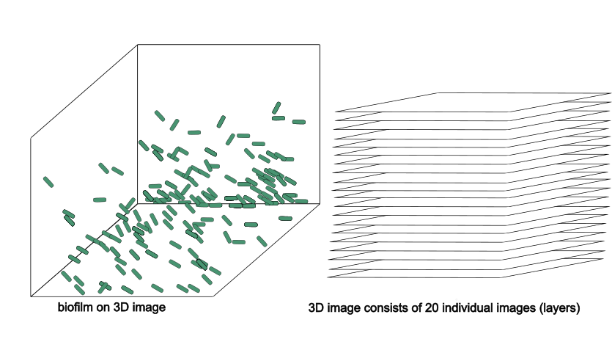
\includegraphics[width=\textwidth]{layers}
	\caption{\label{fig:layers} Schematic representation of input images. Green rods on the left image represent bacteria within the biofilm. }
\end{figure}

Image analysis usually involves some pre-processing steps to distinguish the background from the foreground and to help to recognise objects in the image. Since these procedures require human input, we try to avoid them. In general, the input for feature calculation is a raw image, but for feature counts the pixel intensity values in the raw image are normalised. Normalisation is done by subtracting each pixel intensity value from the average pixel intensity of that layer and then dividing by the difference between maximum and minimum pixel intensity (x - average) / (max - min) to adjust the range of pixel values in an image to a standard range, which here is between 0 and 1. If the feature name in the data file contains “Norminten”, the image has been normalised; if the raw image was taken as input, this is not the case.

All features provide a value for each image but are calculated in two different ways: a) the feature is computed immediately for the whole image or b) the layers are first considered individually and then a value per image is obtained by aggregating the layer values by computing the mean (mean), median (med), standard deviation (std), variance (var) and quantiles (q10, q25, q75 and q90). If the feature is aggregated in the data file, this is noted as \_mean, \_med, \_min, \_max, \_std, \_var, \_q10, \_q25, \_q75, \_q90 at the end of the feature's name. In addition, we also introduce normalised values of features that are calculated for each layer as described later. 

Below you will find descriptions of the features. Appendix~\ref{apdx:features} lists the abbreviations from the data file, the full names of the features, the processing steps and brief explanations. 

\subsection{Morphological features}
These features capture geometric aspects of the biofilm components.

“Biovolume” is the most commonly used feature in the biofilm community, where the number of pixels belonging to the biofilm is counted and then multiplied by the voxel size (here 0.13x0.13x0.5 µm). A threshold is set before counting the pixels and only pixels above this threshold are counted. We generate multiple intensity thresholds, resulting in many biovolume features that differ only by the threshold, so the algorithm must capture the values relevant for classification. This feature is calculated for the image as a whole and not per layers.

The “count" features give the number of bacteria on each layer. For this, a threshold is applied and then the biofilm components (here bacteria) are segmented using the connected components approach from Scipy Multidimensional Image Processing (scipy.ndimage). The objects are then counted for each layer and the counts per layer are aggregated to obtain one value per image. We generate multiple intensity thresholds, resulting in many count features that differ only by the threshold value, so that the algorithm can capture the relevant values for classification. The normalized values of the counts are calculated as described earlier. Although counts intuitively reflect the amount of bacteria, they are based on thresholding and only represent bacteria detected above that threshold, which may not capture all bacteria optimally. 

Substratum Relative Coverage: Percentage of surface covered by biofilm in the 1st layer (surface of the well) of the image.


\subsection{The statistics-based intensity features}

The feature “globalMean” is extracted from the entire 3D image by calculating the average value of all pixel intensity values in the 3D image and is not derived layer by layer (Figure~\ref{fig:layers2}). 

A set of intensity-based features labeled “maxdiffs”, “mindiffs”, “mdiffs” is calculated from the differences of the average pixel intensity values between two consecutive layers, i.e. the average value of the first layer is subtracted from the average value of the second layer and so on until 19 differences are obtained (Figure~\ref{fig:layers2}). Then the maximum, minimum and medium differences are selected and labeled as “maxdiffs”, “mindiffs”, “mdiffs” and given as individual values for each image.


\begin{figure}
	\centering
	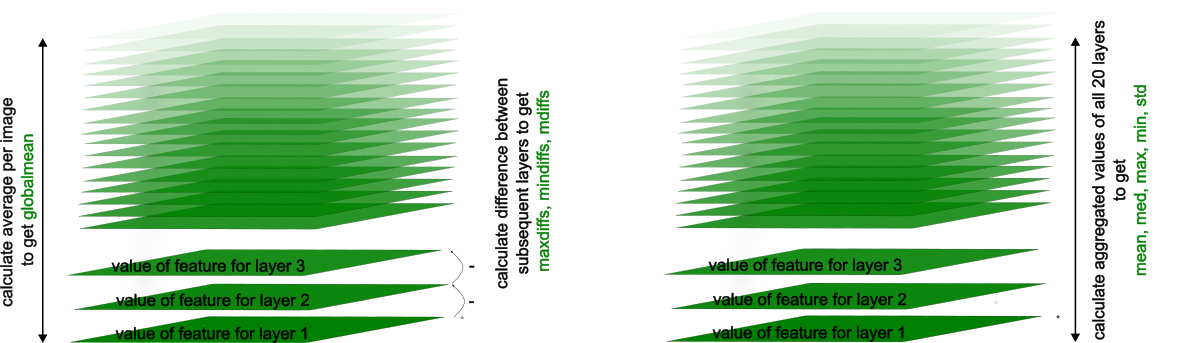
\includegraphics[width=\textwidth]{layers2}
	\caption{\label{fig:layers2} Schematic representation of calculation of intensity-based features.}
\end{figure}

The features “diff” and “diffNormalized” are calculated by subtracting the maximum pixel intensity value from the minimum pixel value for each layer separately. Consequently, we obtain several values for a feature (one per layer), which we combine into a single value by aggregation. In addition, we also introduce normalized features that are calculated for each layer, where the values are normalized by dividing the feature value for the individual layer by the sum of the values calculated for that layer. For example, the maximum difference in pixel intensity on layer 1 is divided by the sum of the maximum differences calculated for layers 1, 2, 3, 4 up to 21. Normalized features are indicated by the presence of “Normalized” in the feature name, e.g. “diffNormalized”.

Another set of intensity-based features labeled “mean”, “med”, “max”, “min” and “std” are calculated by computing the mean, median, maximum, minimum or standard deviation of the pixel intensity values for each layer, and these values are then aggregated. Normalized values are also calculated for these features by calculating the proportion for each layer.

\subsection{Texture features}
Texture features provide a description of an image that contains information about the spatial distribution of pixel intensity values.
“MinProp” is calculated by counting the number of pixels in a layer whose pixel intensity value is below the average pixel intensity value in that layer. This feature is calculated separately for each layer and then aggregated for the entire image as described above. Normalized values are available as “MinPropNormalized”. This feature describes the empty space of the image that is not occupied by bacteria.

The “Homogeneity” is calculated based on the co-occurrence matrix, which represents the distribution of changes in the pixel intensity values of neighboring pixels in the X, Y and Z directions. The formula for calculating homogeneity has already been described1. It measures the similarity of image structures that are spatially close to each other: a higher homogeneity indicates a more homogeneous image structure. This feature is calculated for the image as a whole. 

“ThicknessThreshold” is calculated by tracking the pixel intensity value of each pixel from the first layer (substrate) in height (along the normal to the substrate) until the pixel intensity value reaches 0. The number of the layer where the pixel intensity value reaches 0 is marked, and then the average value of these layers (heights) is calculated. One value is calculated per image.

“roughnessThreshold” is calculated by measuring the height differences for consecutive pixels calculated for "ThicknessThreshold" and then calculating the average. It reflects the height differences of the biofilm.

“Spreading” refers to the spread of the biofilm volume in the 3D image and is calculated as described before2. Three different values are calculated: horizontal spreading (in xy-direction), "Sxy", vertical spreading (in z-direction), "Sz", and total spreading (in xyz-space).

\subsection{Large language model (LLM) based features (GPT features)}

GPT volume refers to the volume of the image layer occupied by the biofilm, where the number of bacteria is multiplied by the voxel size and then aggregated per image.

GPT fractal dimension captures the complexity of the geometric patterns on each image layer and is then aggregated into a single value.
"GPTContrast",” “GPTDissimilarity",” “GPTHomogeneity",” “GPTEnergy",” “GPTCorrelation” and “GPTASM" were calculated using the Graycomatrix method. In this method, a gray- level co-occurrence matrix (GLCM) is created by counting how often a pixel with intensity i occurs in a specific spatial relationship to a pixel with intensity j. The correlation measures, for example, how strongly pairs of grey levels vary together, which indicates predictable spatial patterns in the image.

GPT correlation: Similar to the Pearson correlation coefficient, the correlation value is calculated based on the correlations between the values in graycomatrix. If the correlations are high, this indicates that certain grey level pairs occur in a predictable manner.

GPT Contrast: The contrast highlights the difference between gray-level values. Larger intensity differences contribute more to the sum, so a higher contrast value indicates greater variability in the intensities of neighbouring pixels.

GPT dissimilarity: Similar to contrast, but it is calculated from absolute differences rather than a squared difference. Dissimilarity also captures local variations in grey levels, but its contribution grows more linearly compared to the quadratic term of contrast.

GPT homogeneity: It is calculated in a very similar way to non-GPT homogeneity, but here it is first calculated per layer and then summarised per image by aggregation. However, a high homogeneity indicates a more uniform and less varied texture.

GPT energy: Energy is another way of expressing the uniformity or regularity of texture. It is often used because it is on a scale of [0,1] when P is normalised. 

\FloatBarrier

\appendix


\section{List and descriptions of biofilm features calculated by the Imagine pipeline\label{apdx:features}}


* The image can be analysed as a raw image without adjustments or the pixel intensity values  can be normalised, which is referred to as norminten. The pixel intensity values  in the  raw image are normalized per layer by subtracting the average pixel intensity value of the individual layer by the sum of average pixel intensity values for all layers to obtain values between 0 and 1.

** All features in the data file are aggregated by calculating the mean, median, maximum, minimum and quartiles 10, 25, 75 and 90, standard deviation and variance across the image layers. If the name of the feature contains "SUMMARY", this means that it is an aggregated value of the feature, and the aggregation type is written after the underscore at the end of the feature name \_mean, \_med, \_min, \_max, \_q10, \_q25, \_q75, \_q90, \_std, \_var.


\begin{landscape}
\begin{figure}
	\centering
	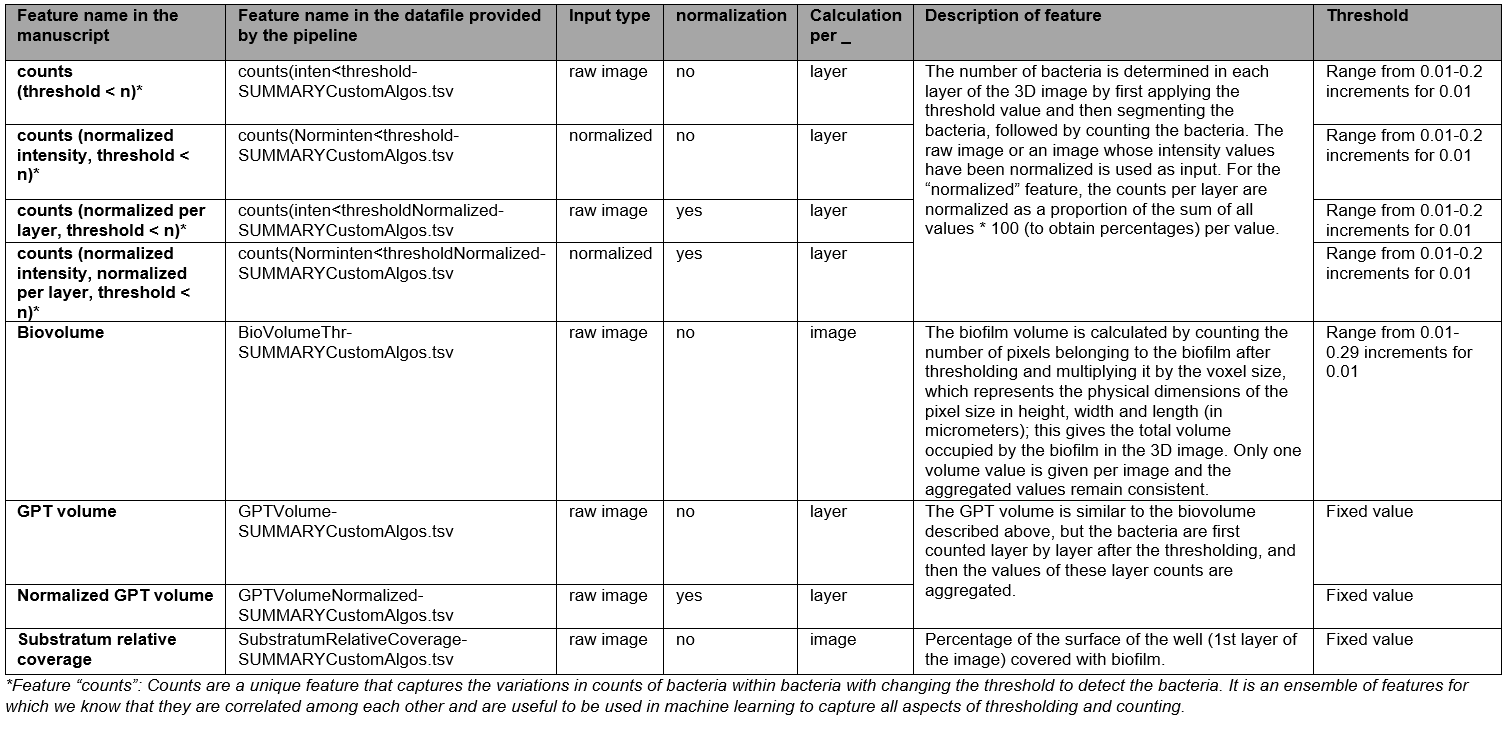
\includegraphics[width=\paperwidth]{morph}
	\caption{\label{fig:morph} Morphological features.}
\end{figure}
\end{landscape}


\begin{landscape}
	\begin{figure}
		\centering
		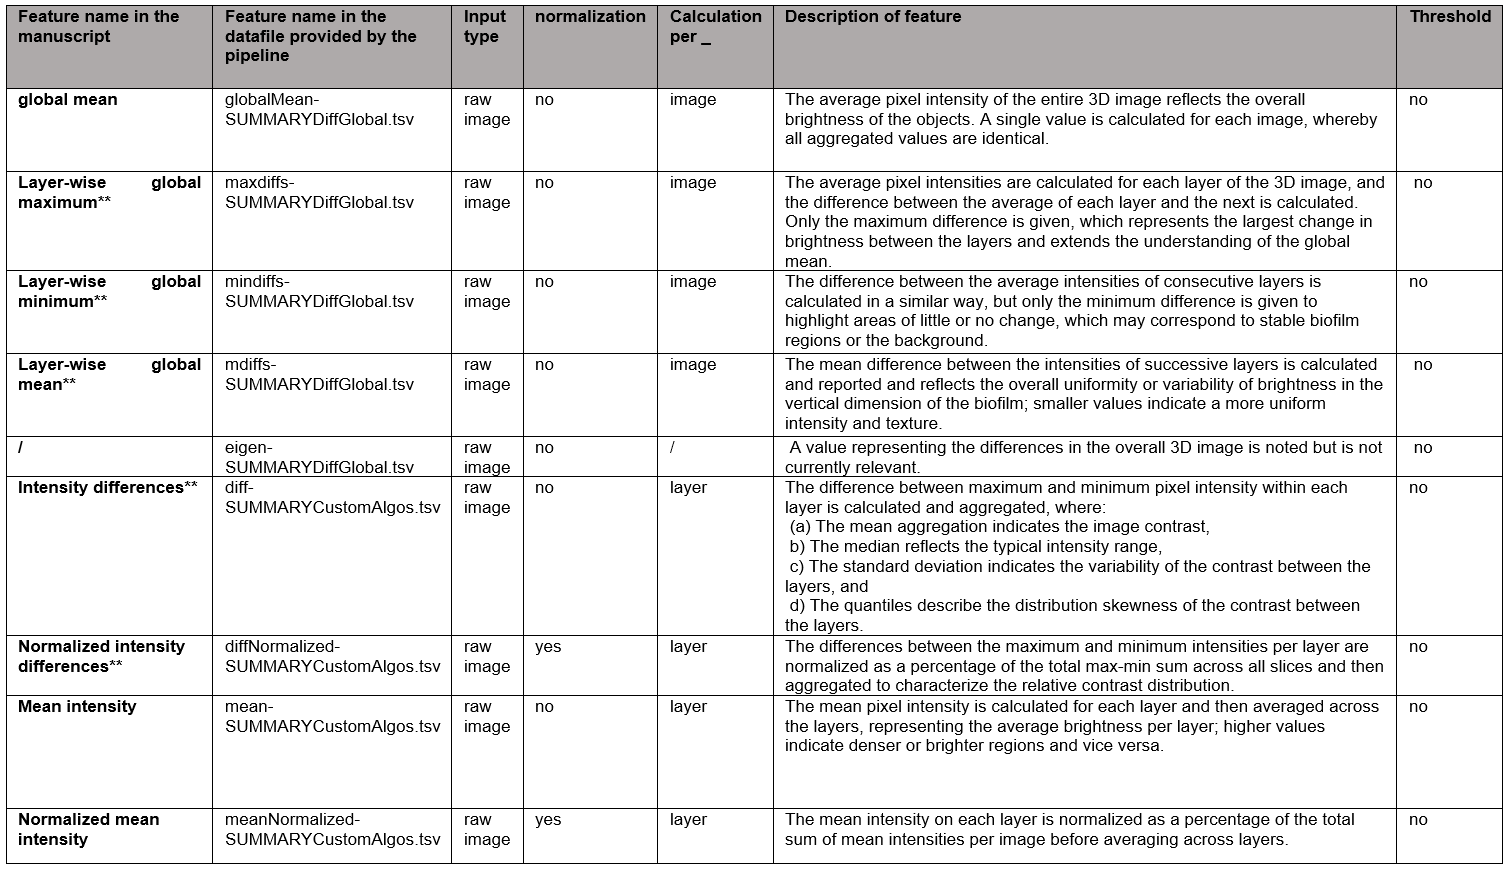
\includegraphics[width=\paperwidth]{stat1}
		\caption{\label{fig:stat1} Statistics-based intensity features (1 of 2).}
	\end{figure}
\end{landscape}

\begin{landscape}
	\begin{figure}
		\centering
		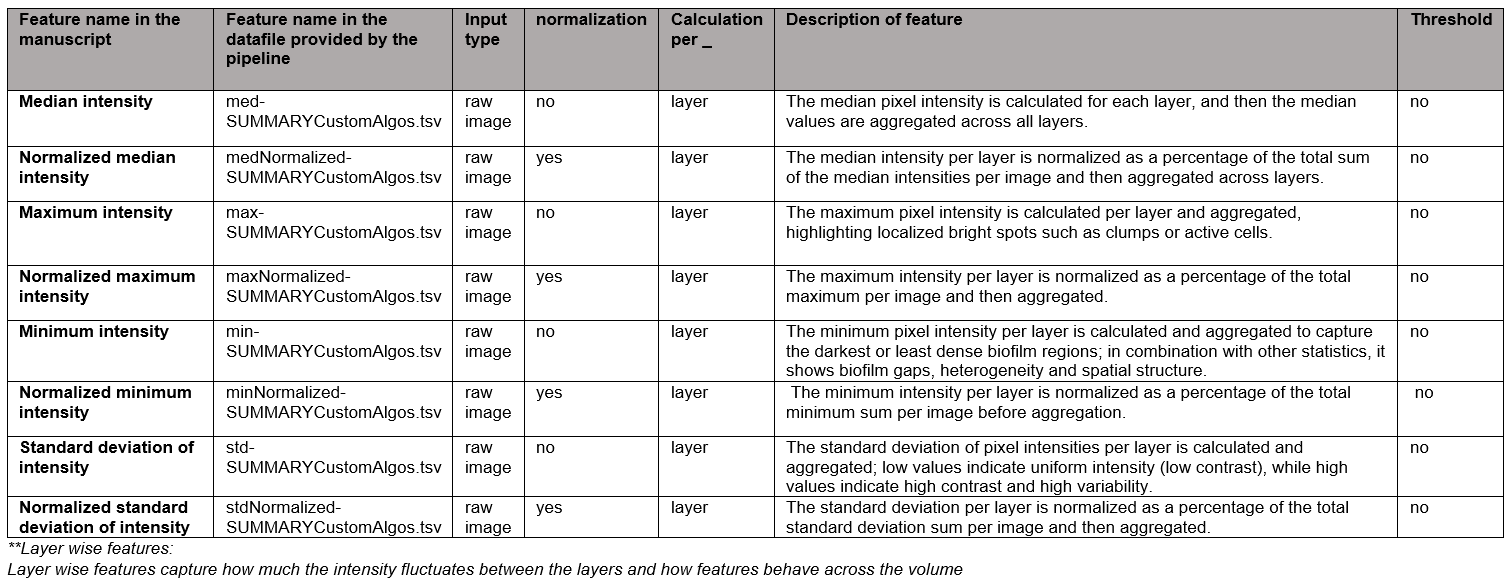
\includegraphics[width=\paperwidth]{stat2}
		\caption{\label{fig:stat2} Statistics-based intensity features (2 of 2).}
	\end{figure}
\end{landscape}

\begin{landscape}
	\begin{figure}
		\centering
		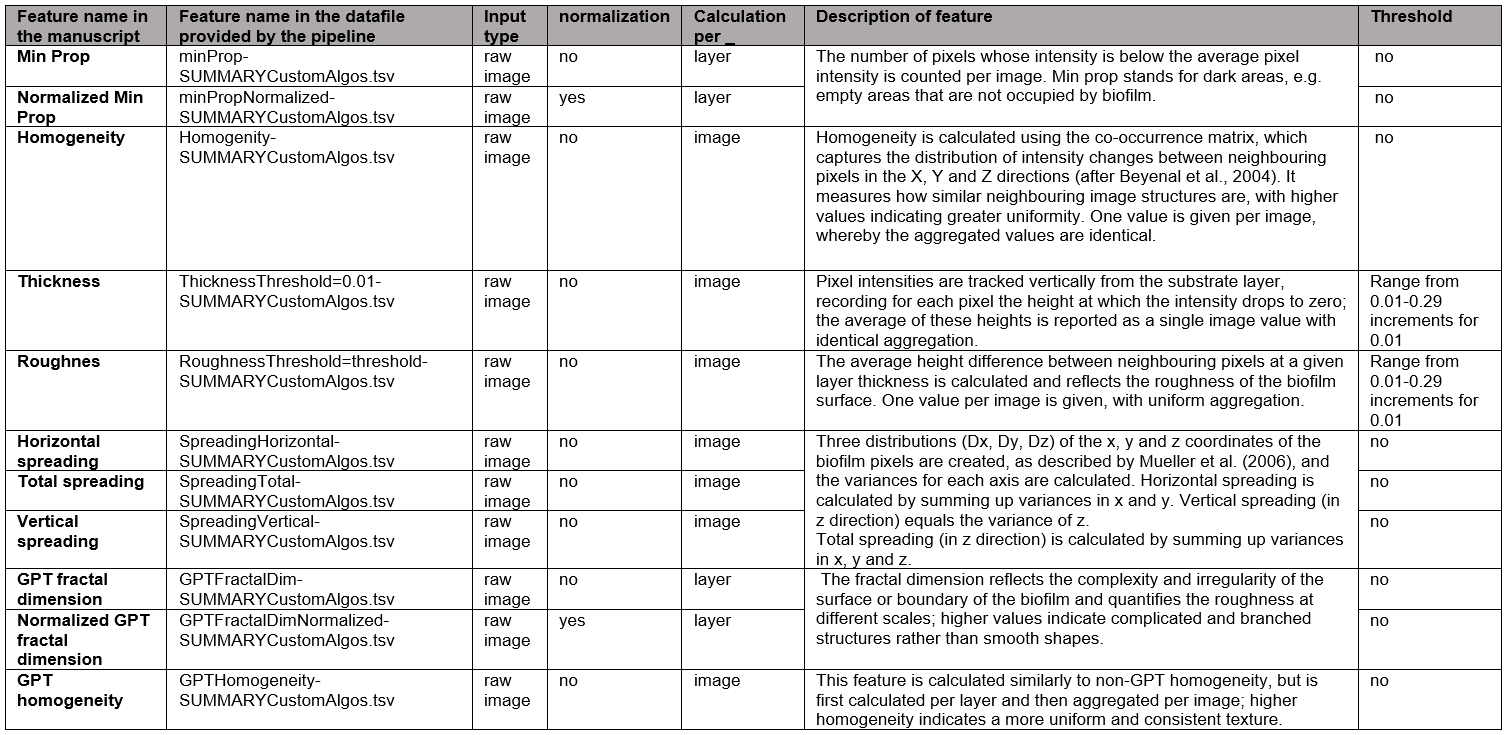
\includegraphics[width=\paperwidth]{texture}
		\caption{\label{fig:texture} Texture features.}
	\end{figure}
\end{landscape}

\begin{landscape}
	\begin{figure}
		\centering
		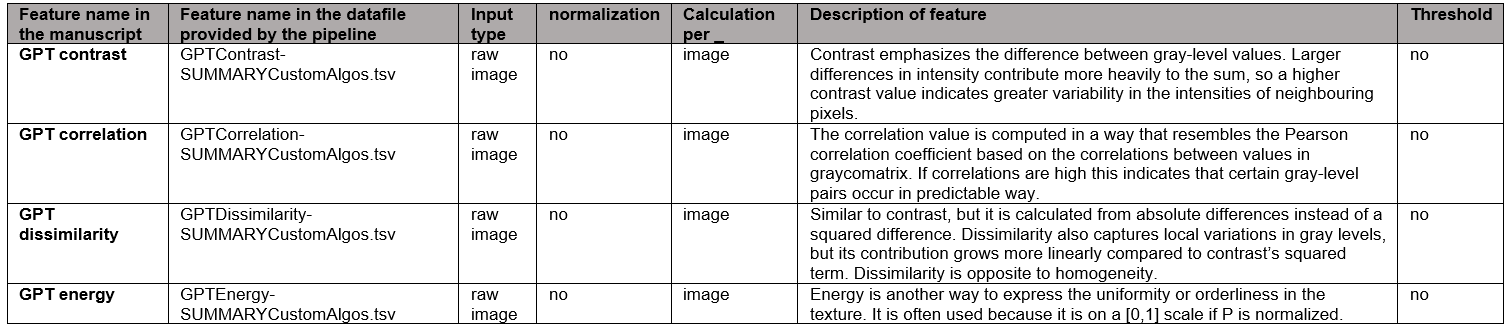
\includegraphics[width=\paperwidth]{graycomatrix}
		\caption{\label{fig:graycomatrix} Graycomatrix method features.}
	\end{figure}
\end{landscape}
\end{document}

